\documentclass[border=8pt]{standalone}
\usepackage{tikz}
\usetikzlibrary{positioning,arrows.meta,fit,calc}
\renewcommand{\familydefault}{\sfdefault}

\definecolor{ink}{HTML}{1F2937}
\definecolor{muted}{HTML}{6B7280}
\definecolor{line}{HTML}{CBD5E1}
\definecolor{inbg}{HTML}{EFF6FF}\definecolor{inbd}{HTML}{3B82F6}
\definecolor{nmbg}{HTML}{F5F3FF}\definecolor{nmbd}{HTML}{7C3AED}
\definecolor{trbg}{HTML}{ECFDF5}\definecolor{trbd}{HTML}{059669}
\definecolor{jgbg}{HTML}{FFF7ED}\definecolor{jgbd}{HTML}{EA580C}
\definecolor{outbg}{HTML}{F8FAFC}\definecolor{outbd}{HTML}{334155}
\definecolor{cq}{HTML}{3B82F6}\definecolor{ct}{HTML}{7C3AED}
\definecolor{co}{HTML}{A78BFA}\definecolor{ce}{HTML}{DC2626}\definecolor{cc}{HTML}{6B7280}

\begin{document}
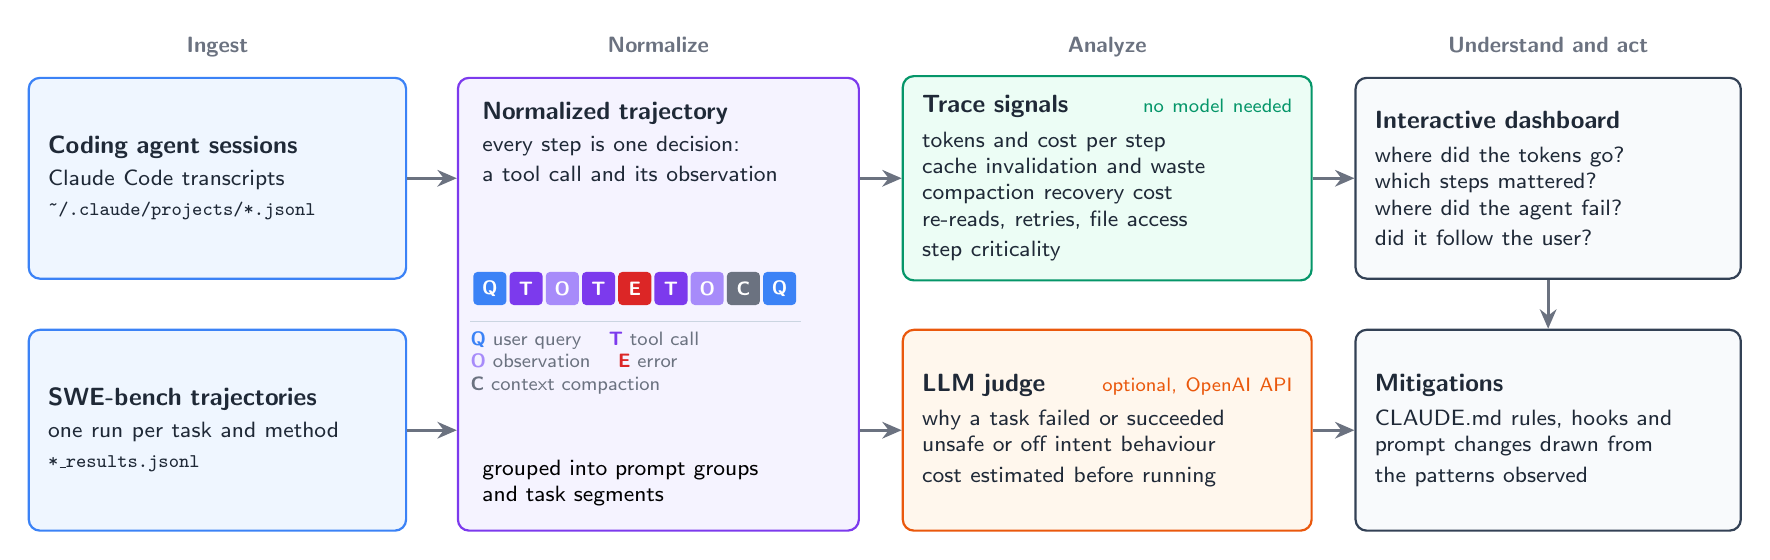
\begin{tikzpicture}[
  font=\small\color{ink},
  box/.style={draw, rounded corners=4pt, line width=0.8pt, align=left, inner sep=7pt, text width=#1, minimum height=2.55cm},
  box/.default=4.3cm,
  head/.style={font=\bfseries\normalsize, anchor=south west, inner sep=0pt},
  stage/.style={font=\footnotesize\bfseries\color{muted}, anchor=base},
  arr/.style={-{Stealth[length=7pt,width=6pt]}, line width=1.1pt, color=muted},
  chip/.style={minimum width=0.42cm, minimum height=0.42cm, inner sep=0pt, rounded corners=1.5pt,
               font=\scriptsize\bfseries\color{white}},
]

% ---------- column 1: inputs ----------
\node[box, draw=inbd, fill=inbg] (cc) at (0,1.6) {%
  \textbf{Coding agent sessions}\\[2pt]
  {\footnotesize Claude Code transcripts\\ \texttt{\scriptsize\textasciitilde/.claude/projects/*.jsonl}}};
\node[box, draw=inbd, fill=inbg] (swe) at (0,-1.6) {%
  \textbf{SWE-bench trajectories}\\[2pt]
  {\footnotesize one run per task and method\\ \texttt{\scriptsize *\_results.jsonl}}};

% ---------- column 2: normalize ----------
\node[box=4.6cm, draw=nmbd, fill=nmbg, minimum height=5.75cm] (norm) at (5.6,0) {};
\node[anchor=north west, align=left, text width=4.2cm] at ($(norm.north west)+(0.2,-0.2)$) {%
  \textbf{Normalized trajectory}\\[2pt]
  {\footnotesize every step is one decision:\\ a tool call and its observation}};
% step strip: Q T O T O E T O | C | Q T O
\begin{scope}[shift={($(norm.west)+(0.42,0.2)$)}]
  \foreach \lab/\col [count=\i] in {Q/cq,T/ct,O/co,T/ct,E/ce,T/ct,O/co,C/cc,Q/cq} {
    \node[chip, fill=\col] at ({(\i-1)*0.46},0) {\lab};
  }
  \draw[line, line width=0.6pt] (-0.25,-0.42) -- (3.95,-0.42);
  \node[anchor=north west, font=\scriptsize\color{muted}, align=left, text width=4.2cm, inner sep=0pt] at (-0.25,-0.55) {%
    \textcolor{cq}{\textbf{Q}} user query \quad \textcolor{ct}{\textbf{T}} tool call\\
    \textcolor{co}{\textbf{O}} observation \quad \textcolor{ce}{\textbf{E}} error\\
    \textcolor{cc}{\textbf{C}} context compaction};
\end{scope}
\node[anchor=south west, align=left, text width=4.2cm, font=\footnotesize] at ($(norm.south west)+(0.2,0.2)$) {%
  grouped into prompt groups\\ and task segments};

% ---------- column 3: analysis ----------
\node[box=4.7cm, draw=trbd, fill=trbg] (trace) at (11.3,1.6) {%
  \textbf{Trace signals}\hfill{\scriptsize\color{trbd}no model needed}\\[3pt]
  {\footnotesize tokens and cost per step\\
   cache invalidation and waste\\
   compaction recovery cost\\
   re-reads, retries, file access\\
   step criticality}};
\node[box=4.7cm, draw=jgbd, fill=jgbg] (judge) at (11.3,-1.6) {%
  \textbf{LLM judge}\hfill{\scriptsize\color{jgbd}optional, OpenAI API}\\[3pt]
  {\footnotesize why a task failed or succeeded\\
   unsafe or off intent behaviour\\
   cost estimated before running}};

% ---------- column 4: outputs ----------
\node[box=4.4cm, draw=outbd, fill=outbg] (dash) at (16.9,1.6) {%
  \textbf{Interactive dashboard}\\[3pt]
  {\footnotesize where did the tokens go?\\
   which steps mattered?\\
   where did the agent fail?\\
   did it follow the user?}};
\node[box=4.4cm, draw=outbd, fill=outbg] (act) at (16.9,-1.6) {%
  \textbf{Mitigations}\\[3pt]
  {\footnotesize CLAUDE.md rules, hooks and\\ prompt changes drawn from\\ the patterns observed}};

% ---------- stage labels ----------
\foreach \nd/\lbl in {cc/Ingest, norm/Normalize, trace/Analyze, dash/Understand and act} {
  \path let \p1=(\nd.north) in node[stage] at (\x1, 3.2) {\lbl};
}

% ---------- arrows (straight, horizontal) ----------
\draw[arr] (cc.east)    -- (cc.east -| norm.west);
\draw[arr] (swe.east)   -- (swe.east -| norm.west);
\draw[arr] (trace.west -| norm.east) -- (trace.west);
\draw[arr] (judge.west -| norm.east) -- (judge.west);
\draw[arr] (trace.east) -- (trace.east -| dash.west);
\draw[arr] (judge.east) -- (judge.east -| act.west);
\draw[arr] (dash.south) -- (act.north);

\end{tikzpicture}
\end{document}
